\section{Flask API}\label{flask-api}

Flask API je implementace stejných webově procházetelných API, které poskytuje Django REST framework \autocite{flaskapi} (o~něm jsem psal \protect\hyperlink{drf:fra}{v~části}), ale bez závislosti na Djangu.

Za projektem stojí autor Django REST frameworku, Tom Christie. Zatím se ale naneštěstí jedná o~rozdělanou práci \autocite{flaskapi} a zdaleka nejde o~hotový projekt. Práce na Flask API je zároveň pozastavená, kvůli závazkům z~crowdfundingové kapaně k~Django REST frameworku \autocite{flaskapigh}. Tom Christie se od roku 2014 (kdy projekt i vznikl) na projektu aktivně nepodílí, existují však další jednotlivci, kteří projekt udržují a rozvíjí.

Pomocí Flask API je nyní možné webově procházet API, jak můžete vidět \protect\hyperlink{pic:flaskapibrowsable}{na obrázku}, ale tvorba API zatím není příliš automatizovaná, \protect\hyperlink{code:flaskapi}{viz příklad}\footnote{Příklad byl mírně zhuštěn za účelem lepší prezentace na straně formátu A4.}.

\begin{figure}
\centering
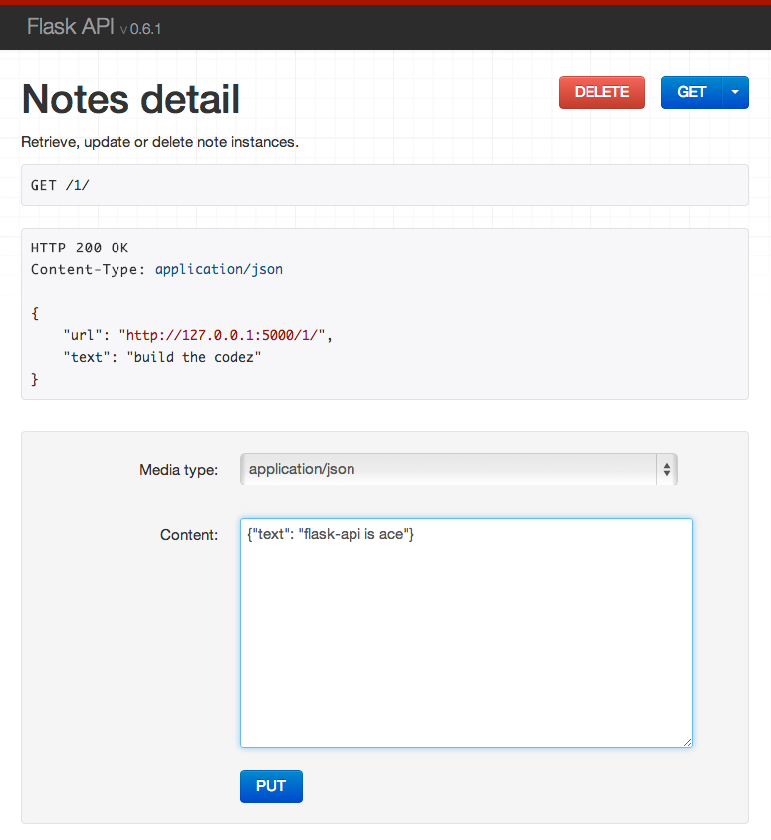
\includegraphics{images/flask-api-browsable}
\caption{Flask API: Webově procházetelné API \autocite{flaskapi}\label{pic:flaskapibrowsable}}
\end{figure}

\begin{listing}[htbp]
\caption{{\label{code:flaskapi}Příklad použití z~dokumentace Flask API \autocite{flaskapigh}}}
\begin{minted}[bgcolor=codebg]{python}
from flask import request, url_for
from flask_api import FlaskAPI, status, exceptions

app = FlaskAPI(__name__)

notes = {
    0: 'do the shopping',
    1: 'build the codez',
    2: 'paint the door',
}

def note_repr(key):
    return {
        'url': request.host_url.rstrip('/') + \
               url_for('notes_detail', key=key),
        'text': notes[key]
    }

@app.route("/", methods=['GET', 'POST'])
def notes_list():
    """List or create notes."""
    if request.method == 'POST':
        note = str(request.data.get('text', ''))
        idx = max(notes.keys()) + 1
        notes[idx] = note
        return note_repr(idx), status.HTTP_201_CREATED

    # request.method == 'GET'
    return [note_repr(idx) for idx in sorted(notes.keys())]

@app.route("/<int:key>/", methods=['GET', 'PUT', 'DELETE'])
def notes_detail(key):
    """Retrieve, update or delete note instances."""
    if request.method == 'PUT':
        note = str(request.data.get('text', ''))
        notes[key] = note
        return note_repr(key)

    elif request.method == 'DELETE':
        notes.pop(key, None)
        return '', status.HTTP_204_NO_CONTENT

    # request.method == 'GET'
    if key not in notes:
        raise exceptions.NotFound()
    return note_repr(key)

if __name__ == "__main__":
    app.run(debug=True)
\end{minted}
\end{listing}

Projekt v~současnosti přímo závisí jen na frameworku Flask, tím má nepřímo pět závislostí a s~nimi 20~938 řádků kódu. Je distribuován pod BSD licencí \autocite{BSD2} a podporuje obě verze Pythonu.

Do budoucna je plánováno \autocite{flaskapi}\autocite{flaskapigh}:

\begin{itemize}
\tightlist
\item
  autentizace, mj. pomocí session, tokenu i jménem a heslem,
\item
  přístupová práva,
\item
  limitování počtu požadavků v~čase,
\item
  API zdroje pomocí tříd,
\item
  vylepšení procházetelných API, například přidání drobečkové navigace,
\item
  možnost vlastního zpracování výjimek,
\item
  ochrana proti CSRF,
\item
  přihlašování a odhlašování přes prohlížeč v~případě procházetelných API,
\item
  zdokumentování validace požadavků a prolinkování.
\end{itemize}

Je však otázka, kdy a jestli se toho dočkáme.

Zatím neexistují žádné automatické mechanismy pro správu přístupových práv či HATEOAS. Flask API tedy za oba aspekty získává nula bodů.
